\chapter{Appendix}

\section{Generating Ions}
\todo{split and move between PI in ch2, and hardware in ch3\\
-Main points:\\
    -Atomic oven \\
        -Really this is just for future members.\\
        -What temperature/current we go to\\
    -PI lasers\\
        -What powers/ saturation/ frequencies we use for trapping\\
        -Concerns of charging the trap with the UV lasers}

\section{Gate Fidelity}
\label{sec:fidelity}
We derive the fidelity of a noisy gate implementation with respect to the ideal unitary.\\
A quantum channel,
\begin{equation}
    \mathcal{E}: \rho \mapsto \rho,
\end{equation}
which executes ideal unitary, $U$, with some error, has 
an average operation fidelity given by, 
\begin{equation}
    \label{eqn:fid}
    F(\mathcal{E},U) = \int d\psi \bra{\psi} U^\dagger \mathcal{E}(\ket{\psi}\bra{\psi}) U \ket{\psi},
\end{equation}
where the integral is taken over the uniform Haar measure on the space of pure states~\cite{bowdrey_fidelity_2002, nielsen_simple_2002}. We shall see that the language used for this analysis of single qubit gate fidelities closely resembles the group theory approach describing randomised benchmarking. The Haar measure is relevant here to consider the fidelity of the operation independent of the initial state (assuming it is pure), which is exactly the enforced criteria through Clifford twirling during RB. For a single qubit, this can be expressed as an integral over the Bloch sphere. 
If we further assume that the error channel is unitary, as is the case of a detuned channel considered here, we shall find that the fidelity follows
\begin{equation}
    \label{eqn:fid_unitary}
    F(V,U) = \frac{1}{d(d+1)} \left( |\text{Tr}(U^\dagger V)|^2 + d \right),
\end{equation}
 where $V$ is the error unitary, and $d$ is the dimension of the Hilbert space. \\
Here we shall give a derivation of this result, by considering the symmetry imposed by the Haar measure.
The standard fidelity of two unitaries following from equation~\ref{eqn:fid} is given by
\begin{equation}
\begin{split}
    F(V,U) &= \int d\psi \bra{\psi} U^\dagger V \ket{\psi}\bra{\psi} V^\dagger U \ket{\psi},\\
    &= \int d\psi |\bra{\psi} W \ket{\psi}|^2,\\
\end{split}
\end{equation}
where $W=U^\dagger V$.
Using the identity $\text{Tr}(A)\text{Tr}(B) = \text{Tr}(A\otimes B)$, we can rewrite the fidelity as a two-copy expectation value,
\begin{equation}
    F(V,U) = \text{Tr}\left( \left(W \otimes W^\dagger\right) \int d\psi \left(\ket{\psi}\bra{\psi}\right)^{\otimes 2}\right),
\end{equation}
where we have now separated the fidelity into a part dependent on the error channel, and a part equivalent to the second moment of the Haar measure, explicitely rewritten as
\begin{equation}
    \mathcal{M}_2 = \int d\psi \left(\ket{\psi}\bra{\psi}\right)^{\otimes 2}.
\end{equation}
We now consider two apparent symmetries of $\mathcal{M}_2$: first, the Haar measure is invariant under unitary transformations, and so our expression must commute with $U \otimes U$ for any unitary $U$; second, the two states in the tensor product are identical, and so $\mathcal{M}_2$ must be invariant under the swap operator $S$ which exchanges the two copies. These two symmetries are sufficient to show that $\mathcal{M}_2$ is proportional to the projector onto the symmetric subspace of the two-copy Hilbert space, which is given by
\begin{equation}
    \Pi_{\text{sym}} = \frac{1}{2}(\mathbb{I} + S).
\end{equation}
To normalise the moment (as the Haar measure is a probability distribution), we enforce $\text{Tr}(\mathcal{M}_2) = 1$. In this two-copy expression, it is apparant that $\text{Tr}(I) = d^2$ and $\text{Tr}(S) = d$, resulting in,
\begin{equation}
    \mathcal{M}_2 = \frac{1}{d(d+1)} \left(\mathbb{I} + S\right). 
\end{equation}
Incorporating this result into the fidelity expression, we find
\begin{equation}
    F(V,U) = \frac{1}{d(d+1)} \text{Tr}\left[ (W \otimes W^\dagger)(\mathbb{I} + S) \right],
\end{equation}
where we can evaluate the two terms using the identities $\text{Tr}(A \otimes B) = \text{Tr}(A)\text{Tr}(B)$ and $\text{Tr}((A \otimes B)S) = \text{Tr}(AB)$, the latter of which is highly relevant to the mechanism of virtual distillation, described in chapter~\ref{ch:virtual_distillation}. This results in the final expression for the fidelity of a unitary error channel with respect to a target unitary, given above by equation~\ref{eqn:fid_unitary}.\\

\section{Projectors of $Cl_1^{\otimes 2}$}
\label{sec:k-copy_projector}
We outline the method of recovering the $\alpha$ parameters described in section~\ref{sec:common_noise} using projectors onto the irrep spaces. A special thanks to Iver Romvig {\O}vergaard who performed this analysis applied to the \emph{common noise} channel and gave permission for reproducing the results here. \\
The decay due to a single rotation acting identically on both qubits which, in the Pauli-transfer matrix (PTM) representation, can be written as $\Lambda^\mathcal{P}=\mathrm{diag}(1, R, R, R\otimes R)$, 
where superscript $\mathcal{P}$ represents the block diagonal matrix is ordered by the two-qubit Pauli basis $\mathcal{P}=\{I\otimes I, \vec\sigma\otimes I , I\otimes\vec\sigma, \vec\sigma\otimes\vec\sigma\}$, with $\vec\sigma = \{\hat\sigma_x, \hat\sigma_y, \hat\sigma_z\}$, and
$R=R(\vec{n}, \theta)\in SO(3)$ describes a rotation by $\theta$ around $\vec{n}$. Finding the vector $\vec\alpha$ can now be done using Schur's lemma for the case of no mixing between irrep spaces:
\begin{equation}\label{eqn:PTM projector decomposition}
    \tilde\Lambda^\mathcal{P}=\sum_\lambda\alpha_\lambda\Pi_\lambda,\hspace{10pt} \alpha_\lambda=\frac{1}{d_\lambda}\mathrm{Tr}(\Pi_\lambda\Lambda^{\mathcal{P}}).
\end{equation}
Here, $\Pi_\lambda$ denotes the PTM projector onto the irrep space labelled $\lambda$ and with dimension $d_\lambda$. It follows immediately that the identity sector is fixed, while the left- and right-qubit sectors produce $\alpha_L=\alpha_R=\mathrm{Tr}(R)/3$. In principle, $\alpha_\lambda$ for the two-qubit sector can be evaluated by explicitly constructing the projectors from the basis operators in Table~\ref{table:irreps}. However, in this case the symmetries of these irrep spaces allow the projectors to be expressed more simply in terms of operators whose traces are easily evaluated:
\begin{align}
\label{eqn:irrep symmetry projector decomposition}
    \Pi_{tr}&=T,\\
    \Pi_{dt}&=D-T,\\
    \Pi_{so}&=\frac{1}{2}(I_9+S)-D,\\
    \Pi_{as}&=\frac{1}{2}(I_9-S),
\end{align}
where $T=1/3\sum_{ij}\ket{ii}\bra{jj}$, $D=\sum_i\ket{ii}\bra{ii}$, and $S=\sum_{ij}\ket{ji}\bra{ij}$ are the trace projector, diagonal projector, and swap operator, respectively. The required traces are
\begin{align}
     \mathrm{Tr}(I_3 R)&=\mathrm{Tr}(R)=(1+2c),\\
     \mathrm{Tr}(I_9(R\otimes R))&=(\mathrm{Tr}(R))^2=(1+2c)^2,\\
    \mathrm{Tr}(T(R\otimes R))&=\frac{1}{3}\mathrm{Tr}(R^TR)=1,\\
    \mathrm{Tr}(D(R\otimes R))&=\sum_i R_{ii}^2=c^2+2c+(1-c)^2\kappa,\\
    \mathrm{Tr}(S(R\otimes R))&=\mathrm{Tr}(R^2)=4c^2-1,
\end{align}
where $c=\cos(\theta)$,  and $\kappa=n_x^4+n_y^4+n_z^4$ is an anisotropy parameter reflecting the fact that Clifford twirling enforces symmetry under permutations of the Pauli axes, rather than under arbitrary rotations. Substituting these traces into equation~\ref{eqn:PTM projector decomposition} and using equation~\ref{eqn:irrep symmetry projector decomposition} yields 
\begin{align}
    \alpha_{L}&=\alpha_R=\alpha_{as}=\frac{1}{3}(1+2c),\\
    \alpha_{tr}&=1,\\
    \alpha_{dt}&=\frac{1}{2}(c^2+2c-1+(1-c)^2\kappa),\\
    \alpha_{so}&=\frac{1}{3}(3c^2-(1-c)^2\kappa).
\end{align}

\section{$ZZ$-type noise}
\label{sec:app_zz_noise}
\begin{figure}
    \begin{center}
    \noindent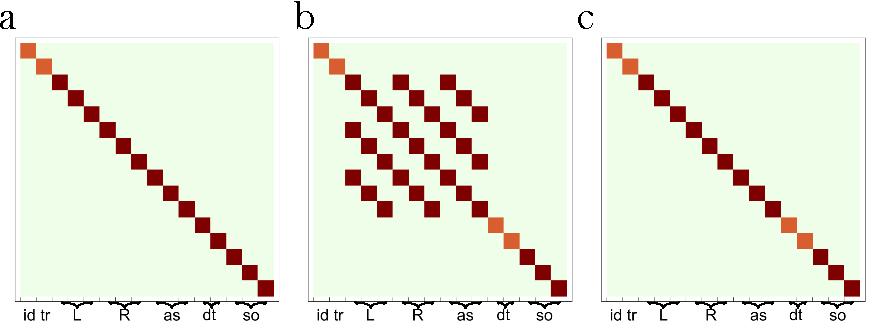
\includegraphics[width=\linewidth]{figures/pdf_figure/ch5/liouville.pdf
        }
    \end{center}
    \caption{
        Liouville operator representation of error channels after twirling over $Cl_1^{\otimes 2}$, ordered by the irrep basis (Schur basis). (a) \emph{Common noise}, (b) Continuous $ZZ$, (c) Stochastic $ZZ$. Orange blocks represent an entry of $1$, green represent $0$, and red represent a decay with dependence on $m$.
        }
    \label{fig:ch4_zz_noise}
\end{figure}
\label{app:zz_err}
In the main text we explore a separable error channel that induces correlations between qubits in a register. Here we shall explore entangling type noise, which although not prevalent on the ion-trap qubit platform, is a dominant error source in superconducting qubits. \\

The always on $ZZ$-type error common to superconducting qubits is described by
the Hamiltonian,
\begin{equation}
\label{eqn:app_HZZ}
H_{ZZ} = \frac{J_{ZZ}}{2}Z\otimes Z,
\end{equation}
where $J_{ZZ}$ is the coupling strength.
Generally, $H_{ZZ}$ will couple
the subrepresentations of the $3$-irrep, given in table~\ref{table:irreps}. We can show the qualitative difference in the subspace dynamics by plotting the Liouville representation of the twirled \emph{common noise}, and the $ZZ$-type noise. Specifically we plot $\tilde\Lambda^m$, where $m$ is the sequence length. Figure~\ref{fig:ch4_fisher_1} plots the maps in the Schur basis
ordered so isotypic representations are adjacent to one another. Orange blocks have entries of $1$, light green blocks are $0$, and red blocks represent some decay parameters dependent on $m$.
Panel (a) shows the fully diagonal \emph{common noise} transfer matrix, where we can see the invariant trace subspace that was noted in the main text. Panel (b) shows the general case for twirled $ZZ$-type noise, given by equation~\ref{eqn:app_HZZ}. The off-diagonal entries exactly couple the three subspaces of the $3$-irrep.
We note that the resulting block diagonal form is inconvenient to express as a
general multi-exponential decay profile as given in the main text for \emph{common} and local depolarising type noise. However, the resulting block diagonal Liouville
form may be used directly with experimental data to fit these parameters of
interest. Further, we may still explore the expected asymptotic decays due to this model, and find that under dominant $ZZ$-type noise, we expect an asymptote of $\mathcal{P}_{SS}|_{m\rightarrow\infty}=1/2$.\\

We may recover a simple diagonal Liouville form in the case of stochastic $ZZ$ noise, given by,
\begin{equation}
\mathcal{E}_{ZZ}(\rho) = (1-p_{ZZ})\rho + p_{ZZ} (Z\otimes Z)\rho(Z\otimes Z),
\end{equation}
where $p_{ZZ}$ is the probability of a correlated phase flip error on both qubits.
In the irrep basis, the following sector decays are found for the stochastic $ZZ$ error,
\begin{equation}
    \begin{split}
        \alpha_L&=\alpha_R=\alpha_{so}=\alpha_{as}= 1- 4p_{ZZ}/3, \\
        \alpha_{tr} &= \alpha_{dt} = 1.\\
    \end{split}
\end{equation}
We show this dependence in figure~\ref{fig:ch4_zz_noise} (c).
The same intermediate asymptote of $\mathcal{P}_{SS}|_{m\rightarrow\infty} = 0.5$ is expected. \\

The difference in correlated decay structure due to \emph{common}, depolarising, and $ZZ$-type errors suggests that twirling over $Cl_1^{\otimes2}$ both simplifies a generic error map to be measurable via RB, but also, retains some noise-dependent structure of the correlated decay profiles.  
Designing optimal initial and final states, as well as optimal sampling strategies for extracting a larger set of error parameters covering multiple physical error mechanisms is left for future work. A possible strategy to avoid introducing arbitrary error channels, is to be agnostic of the physical error mechanisms, and rather directly extract the $\vec\alpha$ and $\vec m$ parameters described in section~\ref{app:reps}. Analogous protocols to this is described by character RB~\cite{helsen_new_2019}, and tomography via RB~\cite{kimmel_robust_2014}.


\section{Magnus expansion}
\label{app:magnus}

    The unitary evolution due to a time dependent Hamiltonian may be written in the ordered, short-time limit as,
    \begin{equation}
        U(t) = \lim_{N\rightarrow\infty} e^{\frac{-i}{\hbar}\hat H(t_N)\Delta t}\cdots e^{\frac{-i}{\hbar}\hat H(t_2)\Delta t}e^{\frac{-i}{\hbar}\hat H(t_1)\Delta t} = e^{A(t)},
    \end{equation}
    where $\Delta t = t/N$, and $t_n = n\Delta t$, and $A(t)$ is a time
    dependent exponent, which is expanded in the Magnus construction to~\cite{magnus_exponential_1954},
    \begin{equation}
        A(t) = \sum_{k=1}^{\infty} A_k(t).
    \end{equation}
    The first three $A_k(t)$ terms are given by,
    \begin{align}
        \label{eqn:magnus_A}
        A_1(t) &= \frac{-i}{\hbar}\int_{0}^{t}dt_1 \hat H(t_1)\\
        A_2(t) &= -\frac{1}{2\hbar^2}\int_{0}^{t}\int_{0}^{t_1}dt_1dt_2 [\hat H(t_1),\hat H(t_2)] \\
        A_3(t) &= \frac{i}{6\hbar^3}\int_{0}^{t}\int_{0}^{t_1}\int_{0}^{t_2}dt_1dt_2dt_3\ \big(\big[\hat H(t_1),\left[\hat H(t_2),\hat H(t_3)\right]\big]+\big[\hat H(t_3),\left[\hat H(t_2),\hat H(t_1)\right]\big]\big),
    \end{align}
    where we can see that if the Hamiltonian fails to commute with itself at different times, the higher-order Magnus terms become relevant.
    This may be understood as the continuous analogy of the Baker-Campbell-Hausdorff formula. It is particularly useful in this thesis to understand the origin of the geometric phase in the MS gate scheme, and the non-linear bosonic interactions generated in the ``two-SDF'' protocol given in~\S~\ref{sec:two-sdf}.

\subsection{Geometric Phase}
\todo{For Geometric phase gates derivation}

\subsection{``Two-SDF'' Dynamics}
    Here we analyse the ``two-SDF'' Hamiltonian given in equation~\ref{eqn:two-sdf} using the Magnus expansion. We recover effective Hamiltonians for both Gaussian interactions, as well as for tri-squeezing. \\
    The ``two-SDF'' Hamiltonian is reproduced for convenience here,
    \begin{align}
      \hat H_\mathrm{2SDF}(t)  &= \hat H_\alpha(t) + \hat H_\beta(t)\\
      &=
      \frac{\hbar \Omega_\alpha}{2}\hat\sigma_\alpha \left(\hat a_\alpha e^{i(\Delta_\alpha t + \phi_\alpha)} + \hat a_\alpha^\dagger e^{-i(\Delta _\alpha t + \phi_\alpha )}\right)\\
      &~+ 
      \frac{\hbar \Omega_{\beta}}{2}\hat\sigma_{\beta} \left(\hat a_\beta e^{i(\Delta_\beta t + \phi_\beta)} + \hat a_\beta^\dagger e^{-i(\Delta_\beta t + \phi_\beta)}\right).
    \end{align}
    The first three terms of the corresponding Magnus expansion are found by inserting $\hat H_\mathrm{2SDF}$ into equations~\ref{eqn:magnus_A}. We shall later rationalise that with certain values of SDF magnitudes, detunings, and phases, we may arbitrarily suppress the higher order terms.\\
    The $A_1$ term appears as separable fast
    oscillations in phase space due to each SDF, 
    \begin{equation}
        A_1(t) = -i\sum_{i\in\{\alpha,\beta\}}\left(\frac{\Omega_i\hat\sigma_i}{\Delta_i}\sin\left(\frac{\Delta_i t}{2}\right)
        \left(\hat a_i e^{i\left(\frac{\Delta_i t}{2} + \phi_i \right)} + \hat a_i^\dagger e^{-i\left(\frac{\Delta_i t}{2} + \phi_i \right)}
        \right)\right).
    \end{equation}
    This is effectively the first-order only dynamics of the displacement operator leading to excursions in phase-space. The effects of this term may be entirely suppressed at certain gate durations, $A_1(T)=0$, where $T$ is an integer multiple of both
    $\tau_\alpha = 2\pi/\Delta_\alpha$ and $\tau_\beta = 2\pi/\Delta_\beta$. Excursions may also be made arbitrarily small by ensuring $\Omega_i \ll \Delta_i$. \\
    The commutator in the $A_2$ term may be expanded to reveal four relevant components,
    \begin{equation}
    A_2(t) = S_\alpha(t) + S_\beta(t) + X_\mathrm{pair}(t) + X_\mathrm{exch}(t),
    \end{equation}
    where $S$ denotes ``self-terms'', and $X$ ``cross-terms'' of the two simultaneously applied SDFs.
    We label the first cross-term ``pair'' due to the pair creation and annihilation of excitations, and the second group, ``exch'' is labelled due to driving the exchange of excitation. \\
    The self-terms, with the form,
    \begin{equation}
        S_i(t) = \frac{i\Omega_i^2}{4}\left(\frac{\sin(\Delta_i t)}{\Delta_i^2} - \frac{t}{\Delta_i}\right)
    \end{equation}
    are recognisable from section~\ref{sec:geometric_phase} as geometric phase factors.
    Taking the assumption that $t\gg \frac{1}{\Delta_i}$, we get a linearly growing geometric phase term,
    $S_i(t) \approx \frac{-i\Omega_i^2t}{4\Delta_i}$.
    In the case that this geometric phase acts globally on the
    system, they may be ignored. If the accumulated phase is spin, or oscillator
    state dependent, then interesting dynamics may be observed, however these
    effects are out of the scope of this thesis. \\
    The remaining cross-terms contain the 2nd order non-linear bosonic interactions we are interested in emulating. 
    We set the two detunings relative to one another by, $\Delta_\beta = m\Delta_\alpha$.
    Expanding the commutator of the cross terms we find for general $m$ the following interactions, grouped by their effect on the oscillator state,
    \begin{align}
        X_\mathrm{pair} &= \frac{i\epsilon_{\alpha\beta\gamma} \Omega_\alpha\Omega_\beta  }{4\Delta }\hat\sigma_\gamma \left(\hat a_\alpha\hat a_\beta e^{i\phi_p}J(m,t)+\hat a_\alpha^{\dagger}a_\beta^\dagger e^{-i\phi_p}J(m,t)^\dagger\right),\\
        X_\mathrm{exch} &= \frac{i\epsilon_{\alpha\beta\gamma}\Omega_\alpha\Omega_\beta }{8\Delta}\left(\{\hat a_\alpha, \hat a_\beta^\dagger\}e^{i\phi_m}F(m,t) + \{\hat a_\alpha^\dagger, \hat a_\beta \} e^{-i\phi_m}F(m,t)^\dagger\right),
    \end{align}
    with $\phi_p = \phi_\alpha + \phi_\beta$, and $\phi_m = \phi_\alpha - \phi_\beta$, and $J$ and $F$ containing resonance like terms,
    \begin{align}
        J(m,t) &=\frac{1-m}{m}\left(\frac{e^{i(m+1)\Delta t}-1}{(m+1)\Delta t}\right)t,\\
        F(m,t) &= \left(\frac{m+1}{m}\frac{e^{-i (m-1)\Delta t}-1}{(m-1)\Delta t} + \frac{e^{i\Delta t}-e^{-im\Delta t}}{m\Delta t}\right)t.
    \end{align}
    We now may find the effective Hamiltonians governing the dynamic evolution for certain resonance conditions.
    We can convert from the generator form, $A(T)$, to familiar effective 
    time-independent Hamiltonian, $\hat H_\mathrm{eff}$ for a given time, $T$, by $\hat H_\mathrm{eff} = \frac{i\hbar}{T}A(T)$.\\
    Taking the limit, $m=-1$, we find $F(-1,t)=0$ and $J(-1,t) = -2it$, leading to a time-linear term $X_\mathrm{pair}$,
    with effective Hamiltonian,
    \begin{equation}
        \hat H_\mathrm{eff, pair} = \frac{\varepsilon_{\alpha\beta\gamma}\hbar \Omega_2}{2}\hat\sigma_\gamma\left(\hat a_\alpha \hat a_\beta e^{i\phi_p'}+\hat a_\alpha^\dagger \hat a_\beta^\dagger e^{-i\phi_p'}\right),
    \end{equation}
    where $\Omega_2 = \frac{\Omega_\alpha\Omega_\beta}{\Delta}$, and $\phi_p' = \phi_\alpha +\phi_\beta + \frac{\pi}{2}$. For $a_\alpha^\dagger = a_\beta^\dagger$ this is the squeezing interaction, whereas for $a_\alpha^\dagger \neq a_\beta^\dagger$ this is two-mode squeezing.\\
    Taking the limit, $m=+1$, we find $J(1,t)=0$ and $F(1,t) = -2it\left(1-\mathrm{sinc}(\Delta t)\right)$. If we consider the secular term only, we find the time-linear term $X_\mathrm{exch}$. Now considering the anticommutation relationships between ladder operators we find for $a_\alpha^\dagger = a_\beta^\dagger$, an effective Hamiltonian,
    \begin{equation}
        \hat H_\mathrm{eff, parity} = \frac{\varepsilon_{\alpha\beta\gamma}\hbar \Omega_2}{2}\hat\sigma_\gamma\sin(\phi_m) (2\hat a_\alpha^\dagger \hat a_\alpha +1),
    \end{equation}
    which is the parity, or in this case ``dispersive'' Hamiltonian due to the spin-conditioning.\\
    Finally, considering $a_\alpha^\dagger \neq a_\beta^\dagger$, we recover the beamsplitter interaction, with effective Hamiltonian,
    \begin{equation}
        \hat H_\mathrm{eff, bs} = \frac{\varepsilon_{\alpha\beta\gamma}\hbar \Omega_2}{2}\hat\sigma_\gamma \left(\hat a_\alpha \hat a_\beta^\dagger e^{i\phi_m'}+\hat a_\alpha^\dagger \hat a_\beta e^{-i\phi_m'}\right),
    \end{equation}
    with $\phi_m' = \phi_\alpha - \phi_\beta + \frac{\pi}{2}$.\\
    Similar arguments hold for the higher order terms, where, for example, we recover the tri-squeezing interaction for $m=-2$, with effective Hamiltonian of the form,
    \begin{equation}
        \hat H_\mathrm{eff, tri} = \frac{\hbar \Omega_3}{2}\hat\sigma_\beta \left(\hat a_\alpha^3 e^{i\phi}+\hat a_\alpha^{\dagger 3}  e^{-i\phi}\right),
    \end{equation}
    with $\Omega_3 = \frac{\Omega_\alpha^2\Omega_\beta}{2\Delta^2}$.\\
    For further details on the use of these higher order effective interactions refer to the following two theses:\cite{bazavan_easy_nodate,saner_quantum_2026}.
    


    \section{Derangement for $k=2$}
    \label{app:derange}
    Huggins~\cite{huggins_virtual_2021} provides a proof of the identity given
    in equation~\ref{eqn:derange}, which I reproduce here for the simple example
    of $k=2$.   The derangement operator for two copies is simply the swap
    operator, $S^{(2)}=\mathrm{SWAP}$, and we will assume the observable acts
    only on the first copy, giving $\hat{O}^1 = \hat{O}\otimes\mathbb{I}$. The
    identity is then,
    \begin{align}
        \mathrm{Tr}[\hat{O}^1S^{(2)}\rho^{\otimes 2}]&\\
        &= \sum_{\substack{i_1,i_2\\j_1,j_2\\k_1,k_2}} \bra{i_1}\hat{O}\ket{k_1}\delta_{i_2,k_2}
        \bra{k_1, k_2}S^{(2)}\ket{j_1,j_2}\bra{j_1}\rho\ket{i_1}\bra{j_2}\rho\ket{i_2}\\
        &= \sum_{\substack{i_1,i_2\\j_1,j_2\\k_1, k_2}} \hat{O}_{i_1, k_1}\delta_{i_2,k_2}\delta_{k_1,j_2}\delta_{k_2,j_1}\rho_{j_1,i_1}\rho_{j_2,i_2}
    \end{align}
    and contracting the Kronecker deltas, we find,
    \begin{align}
        \mathrm{Tr}[\hat{O}^1S^{(2)}\rho^{\otimes 2}]&\\
        &= \sum_{\substack{i_1,j_1, j_1}} \hat{O}_{i_1, j_2}\rho_{j_1,i_1}\rho_{j_2,j_1}\\
        &= \mathrm{Tr}[\hat{O}\rho^2],
    \end{align}
    with the last equality following from the definition of matrix multiplication. \\